\documentclass[a4paper,11pt]{book}
%\documentclass[a4paper,twoside,11pt,titlepage]{book}
\usepackage{listings}
\usepackage[utf8]{inputenc}
\usepackage[spanish]{babel}

% \usepackage[style=list, number=none]{glossary} %
%\usepackage{titlesec}
%\usepackage{pailatino}

\decimalpoint
\usepackage{dcolumn}
\newcolumntype{.}{D{.}{\esperiod}{-1}}
\makeatletter
\addto\shorthandsspanish{\let\esperiod\es@period@code}
\makeatother


%\usepackage[chapter]{algorithm}
\RequirePackage{verbatim}
%\RequirePackage[Glenn]{fncychap}
\usepackage{fancyhdr}
\usepackage{graphicx}
\usepackage{afterpage}

\usepackage{longtable}

\usepackage[pdfborder={000}]{hyperref} %referencia

% ********************************************************************
% Re-usable information
% ********************************************************************
\newcommand{\myTitle}{Título del proyecto\xspace}
\newcommand{\myDegree}{Grado en ...\xspace}
\newcommand{\myName}{Nombre Apllido1 Apellido2 (alumno)\xspace}
\newcommand{\myProf}{Nombre Apllido1 Apellido2 (tutor1)\xspace}
\newcommand{\myOtherProf}{Nombre Apllido1 Apellido2 (tutor2)\xspace}
%\newcommand{\mySupervisor}{Put name here\xspace}
\newcommand{\myFaculty}{Escuela Técnica Superior de Ingenierías Informática y de
Telecomunicación\xspace}
\newcommand{\myFacultyShort}{E.T.S. de Ingenierías Informática y de
Telecomunicación\xspace}
\newcommand{\myDepartment}{Departamento de ...\xspace}
\newcommand{\myUni}{\protect{Universidad de Granada}\xspace}
\newcommand{\myLocation}{Granada\xspace}
\newcommand{\myTime}{\today\xspace}
\newcommand{\myVersion}{Version 0.1\xspace}


\hypersetup{
pdfauthor = {\myName (email (en) ugr (punto) es)},
pdftitle = {\myTitle},
pdfsubject = {},
pdfkeywords = {palabra_clave1, palabra_clave2, palabra_clave3, ...},
pdfcreator = {LaTeX con el paquete ....},
pdfproducer = {pdflatex}
}

%\hyphenation{}


%\usepackage{doxygen/doxygen}
%\usepackage{pdfpages}
\usepackage{xurl}


\usepackage{colortbl,longtable}
\usepackage[stable]{footmisc}
%\usepackage{index}

%\makeindex
%\usepackage[style=long, cols=2,border=plain,toc=true,number=none]{glossary}
% \makeglossary

% Definición de comandos que me son tiles:
%\renewcommand{\indexname}{Índice alfabético}
%\renewcommand{\glossaryname}{Glosario}

\pagestyle{fancy}
\fancyhf{}
\fancyhead[LO]{\leftmark}
\fancyhead[RE]{\rightmark}
\fancyhead[RO,LE]{\textbf{\thepage}}
\renewcommand{\chaptermark}[1]{\markboth{\textbf{#1}}{}}
\renewcommand{\sectionmark}[1]{\markright{\textbf{\thesection. #1}}}

\setlength{\headheight}{1.5\headheight}

\newcommand{\HRule}{\rule{\linewidth}{0.5mm}}
%Definimos los tipos teorema, ejemplo y definición podremos usar estos tipos
%simplemente poniendo \begin{teorema} \end{teorema} ...
\newtheorem{teorema}{Teorema}[chapter]
\newtheorem{ejemplo}{Ejemplo}[chapter]
\newtheorem{definicion}{Definición}[chapter]

\definecolor{gray97}{gray}{.97}
\definecolor{gray75}{gray}{.75}
\definecolor{gray45}{gray}{.45}
\definecolor{gray30}{gray}{.94}

\lstset{ frame=Ltb,
     framerule=0.5pt,
     aboveskip=0.5cm,
     framextopmargin=3pt,
     framexbottommargin=3pt,
     framexleftmargin=0.1cm,
     framesep=0pt,
     rulesep=.4pt,
     backgroundcolor=\color{gray97},
     rulesepcolor=\color{black},
     %
     stringstyle=\ttfamily,
     showstringspaces = false,
     basicstyle=\scriptsize\ttfamily,
     commentstyle=\color{gray45},
     keywordstyle=\bfseries,
     %
     numbers=left,
     numbersep=6pt,
     numberstyle=\tiny,
     numberfirstline = false,
     breaklines=true,
   }
 
% minimizar fragmentado de listados
\lstnewenvironment{listing}[1][]
   {\lstset{#1}\pagebreak[0]}{\pagebreak[0]}

\lstdefinestyle{CodigoC}
   {
	basicstyle=\scriptsize,
	frame=single,
	language=C,
	numbers=left
   }
\lstdefinestyle{CodigoC++}
   {
	basicstyle=\small,
	frame=single,
	backgroundcolor=\color{gray30},
	language=C++,
	numbers=left
   }

 
\lstdefinestyle{Consola}
   {basicstyle=\scriptsize\bf\ttfamily,
    backgroundcolor=\color{gray30},
    frame=single,
    numbers=none
   }


\newcommand{\bigrule}{\titlerule[0.5mm]}


%Para conseguir que en las páginas en blanco no ponga cabecerass
\makeatletter
\def\clearpage{%
  \ifvmode
    \ifnum \@dbltopnum =\m@ne
      \ifdim \pagetotal <\topskip
        \hbox{}
      \fi
    \fi
  \fi
  \newpage
  \thispagestyle{empty}
  \write\m@ne{}
  \vbox{}
  \penalty -\@Mi
}
\makeatother

\usepackage{pdfpages}
\begin{document}
\begin{titlepage}
 
 
\newlength{\centeroffset}
\setlength{\centeroffset}{-0.5\oddsidemargin}
\addtolength{\centeroffset}{0.5\evensidemargin}
\thispagestyle{empty}

\noindent\hspace*{\centeroffset}\begin{minipage}{\textwidth}

\centering

\includegraphics[width=0.9\textwidth]{imagenes/logo_ugr.jpg}\\[1.4cm]

\textsc{ \Large TRABAJO FIN DE GRADO\\[0.2cm]}
\textsc{ INGENIERÍA EN INFORMÁTICA}\\[1cm]
% Upper part of the page
% 
% Title
{\Huge\bfseries PneumologyIOT\\
}
\noindent\rule[-1ex]{\textwidth}{3pt}\\[3.5ex]
{\large\bfseries IOT4CARE: IoT platform for remote
monitoring in care settings}
\end{minipage}

\vspace{2.5cm}
\noindent\hspace*{\centeroffset}\begin{minipage}{\textwidth}
\centering

\textbf{Autor}\\ {Pablo Morenilla Pinos}\\[2.5ex]
\textbf{Directores}\\
{Oresti Baños Legrán\\[2cm]

\includegraphics[width=0.3\textwidth]{imagenes/etsiit_logo.png}\\[0.1cm]
\textsc{Escuela Técnica Superior de Ingenierías Informática y de Telecomunicación}\\
\textsc{---}\\
}
Granada, abril de 2023
\end{minipage}
%\addtolength{\textwidth}{\centeroffset}
%\vspace{\stretch{2}}
\end{titlepage}



\chapter*{}
%\thispagestyle{empty}
%\cleardoublepage

%\thispagestyle{empty}

\begin{titlepage}
 
 
\setlength{\centeroffset}{-0.5\oddsidemargin}
\addtolength{\centeroffset}{0.5\evensidemargin}
\thispagestyle{empty}

\noindent\hspace*{\centeroffset}\begin{minipage}{\textwidth}

\centering
%
\includegraphics[width=0.9\textwidth]{imagenes/logo_ugr.jpg}\\[1.4cm]

%\textsc{ \Large PROYECTO FIN DE CARRERA\\[0.2cm]}
%\textsc{ INGENIERÍA EN INFORMÁTICA}\\[1cm]
% Upper part of the page
% 

 \vspace{3.3cm}

%si el proyecto tiene logo poner aquí

\includegraphics{imagenes/logo.png} 
 \vspace{0.5cm}

% Title

{\Huge\bfseries Título del proyecto\\
}
\noindent\rule[-1ex]{\textwidth}{3pt}\\[3.5ex]
{\large\bfseries Subtítulo del proyecto.\\[4cm]}
\end{minipage}

\vspace{2.5cm}
\noindent\hspace*{\centeroffset}\begin{minipage}{\textwidth}
\centering

\textbf{Autor}\\ {Nombre Apellido1 Apellido2 (alumno)}\\[2.5ex]
\textbf{Directores}\\
{Nombre Apellido1 Apellido2 (tutor1)\\
Nombre Apellido1 Apellido2 (tutor2)}\\[2cm]
%
\includegraphics[width=0.15\textwidth]{imagenes/tstc.png}\\[0.1cm]
%\textsc{Departamento de Teoría de la Señal, Telemática y Comunicaciones}\\
%\textsc{---}\\
%Granada, mes de 201
\end{minipage}
%\addtolength{\textwidth}{\centeroffset}
\vspace{\stretch{2}}

 
\end{titlepage}






\cleardoublepage
\thispagestyle{empty}

\begin{center}
{\large\bfseries Título del Proyecto: Subtítulo del proyecto}\\
\end{center}
\begin{center}
Nombre Apellido1 Apellido2 (alumno)\\
\end{center}

%\vspace{0.7cm}
\noindent{\textbf{Palabras clave}: palabra\_clave1, palabra\_clave2, palabra\_clave3, ......}\\

\vspace{0.7cm}
\noindent{\textbf{Resumen}}\\

Poner aquí el resumen.
\cleardoublepage


\thispagestyle{empty}


\begin{center}
{\large\bfseries Project Title: Project Subtitle}\\
\end{center}
\begin{center}
First name, Family name (student)\\
\end{center}

%\vspace{0.7cm}
\noindent{\textbf{Keywords}: Keyword1, Keyword2, Keyword3, ....}\\

\vspace{0.7cm}
\noindent{\textbf{Abstract}}\\

Write here the abstract in English.

\chapter*{}
\thispagestyle{empty}

\noindent\rule[-1ex]{\textwidth}{2pt}\\[4.5ex]

Yo, \textbf{Nombre Apellido1 Apellido2}, alumno de la titulación TITULACIÓN de la \textbf{Escuela Técnica Superior
de Ingenierías Informática y de Telecomunicación de la Universidad de Granada}, con DNI XXXXXXXXX, autorizo la
ubicación de la siguiente copia de mi Trabajo Fin de Grado en la biblioteca del centro para que pueda ser
consultada por las personas que lo deseen.

\vspace{6cm}

\noindent Fdo: Nombre Apellido1 Apellido2

\vspace{2cm}

\begin{flushright}
Granada a X de mes de 201 .
\end{flushright}


\chapter*{}
\thispagestyle{empty}

\noindent\rule[-1ex]{\textwidth}{2pt}\\[4.5ex]

D. \textbf{Nombre Apellido1 Apellido2 (tutor1)}, Profesor del Área de XXXX del Departamento YYYY de la Universidad de Granada.

\vspace{0.5cm}

D. \textbf{Nombre Apellido1 Apellido2 (tutor2)}, Profesor del Área de XXXX del Departamento YYYY de la Universidad de Granada.


\vspace{0.5cm}

\textbf{Informan:}

\vspace{0.5cm}

Que el presente trabajo, titulado \textit{\textbf{Título del proyecto, Subtítulo del proyecto}},
ha sido realizado bajo su supervisión por \textbf{Nombre Apellido1 Apellido2 (alumno)}, y autorizamos la defensa de dicho trabajo ante el tribunal
que corresponda.

\vspace{0.5cm}

Y para que conste, expiden y firman el presente informe en Granada a X de mes de 201 .

\vspace{1cm}

\textbf{Los directores:}

\vspace{5cm}

\noindent \textbf{Nombre Apellido1 Apellido2 (tutor1) \ \ \ \ \ Nombre Apellido1 Apellido2 (tutor2)}

\chapter*{Agradecimientos}
\thispagestyle{empty}

       \vspace{1cm}


Poner aquí agradecimientos...


%\frontmatter
\tableofcontents
\listoffigures
\renewcommand{\listtablename}{Índice del documento}
\listoftables
%
%\mainmatter
%\setlength{\parskip}{5pt}


\chapter{Introducción.}


\vskip 0.1in

En este trabajo, nos vamos a centrar en el centro hospitalario de Granada (Andalucía, España), Virgen de las Nieves.

En la actualidad, el centro hospitalario mencionado anteriormente no cuenta con un sistema capaz de monitorizar y estudiar el estado ambiental de una habitación de un paciente, requiere de una persona física que se encargue de comprobar que las habitaciones tienen un estado óptimo para el paciente.

No es el caso, puesto que tendría que estar en constante trabajo revisando todas las habitaciones permanentemente y por no mencionar que, hay muchos casos que no puede evaluar una persona con sólo sus sentidos.

Se requiere el uso de medios electrónicos e informáticos para poder saber ciertamente si una habitación de un paciente está en buenas condiciones o, por el contrario, que se actúe.

Una persona puede valorar si la temperatura es la adecuada, pero ¿cómo podría valorar el nivel de $CO_2$, partículas $PM2.5$ u otros elementos ambientales que son indetectables y no pueden ser analizados si no se usan las herramientas adecuadas?

Este proyecto tiene como fin arreglar este problema: «Hacer una IoT de medicina para las habitaciones de los pacientes de la planta de neumología del hospital Virgen de las Nieves». Capaz de poder monitorizar el estado ambiental y detectar si está en condiciones adecuadas o presentan algún problema, de este modo, se evita el depender del personal que revise todas las habitaciones y se estudian las habitaciones sin depender de percepciones subjetivas de personas.

%
%Cómo se podrían automatizar y hacer una IoT de medicina para las habitaciones de los pacientes, en este caso se quiere trabajar con la planta de neumología. 

%\vskip 0.1in

%Puesto que están en constante exposición a posibles peligros ambientales que pueden hacer que empeore su salud y estos valores no se pueden analizar por medio de los componentes médicos que poseen los hospitales, pues estos, miden al paciente pero no al estado de la habitación del paciente.

%\vskip 0.1in

%La idea es poder estudiar el estado ambiental de una habitación de hospital para poder evaluar si corre algún peligro o necesita que se haga alguna acción, ya sea de manera automática con los dispositivos de este proyecto o bien sea por medio de una notificación
%al médico, enfermero u otro responsable de la planta de neumología.

\newpage

\section{Hospitales.}

    Vamos a detallar en este apartado, cómo son las habitaciones de los pacientes, sobre qué normativas están reguladas y qué organización o entidad es la encargada de regular/valorar el estado/calidad de un centro hospitalario en Andalucía.
    
    \vskip 0.2in
    {\large \textbf{Características.}}
    \vskip 0.2in
    
    Para poder ver primero cómo son las habitaciones de los hospitales, hay que ver primero sobre qué estándar o sobre qué criterios se basan los hospitales. 
    
    Depende de distintos factores: país, tipo de centro sanitario, privado, público, fecha de creación, especialidad del mismo, tamaño total del centro hospitalario, entre otros. Para este documento y el desarrollo del proyecto nos vamos a centrar en los hospitales y centros sanitarios de España, concretamente en Andalucía y la provincia de Granada.

    \vskip 0.2in
    {\large \textbf{Implementación de las normativas.}}
    \vskip 0.2in

    Las normativas que regulan las habitaciones de los hospitales para pacientes pueden variar según la ubicación geográfica, pero por lo general, se rigen por regulaciones y estándares emitidos por agencias gubernamentales de salud, así como por organizaciones internacionales y nacionales de acreditación de atención médica.
    
    \vskip 0.1in

    En los Estados Unidos, la Comisión Conjunta es una organización acreditadora de atención médica que establece estándares para la seguridad y calidad de la 
    atención médica. 

    \vskip 0.1in
    
    La Comisión Conjunta tiene una serie de estándares específicos para los entornos físicos de atención médica, que incluyen los requisitos para las habitaciones de los pacientes. Estos estándares se conocen como los Estándares de Acreditación de la Comisión Conjunta.

    \vskip 0.1in

    En otros países, existen organizaciones similares que establecen normativas y estándares para la atención médica, como el Consejo Internacional de Enfermeras, la Organización Mundial de la Salud y la Agencia de Calidad de Atención Sanitaria en España, siendo esta última en la que vamos a fijarnos y analizar sus estándares.

    \newpage
    \vskip 0.2in
    {\large \textbf{Agencia de Calidad Sanitaria de Andalucía (ACSA).}}
    \vskip 0.2in

        Tal como se menciona en la propia página web de ACSA\cite{ACSA_Quienes_Son}: 
        \vskip 0.15in

        La Agencia de Calidad Sanitaria de Andalucía (ACSA) es una organización pública de evaluación y certificación adscrita a la Consejería de Salud y Consumo de la Junta de Andalucía e integrada en la Fundación Progreso y Salud\cite{ACSA_Quienes_Son}. 

        \vskip 0.1in
        
        Su finalidad es impulsar la cultura de la calidad y la mejora continua de los servicios que prestan las organizaciones y los profesionales sanitarios y de servicios sociales, reto que la ACSA afronta ofreciendo herramientas y servicios específicos, buscando siempre la excelencia en la atención a la salud y el bienestar social\cite{ACSA_Quienes_Son}.

        \vskip 0.1in

        Para ello, se erige como entidad certificadora de la calidad de organizaciones sanitarias y de servicios sociales, así como de sus profesionales y de la formación que estos reciben. Así, la ACSA acompaña a las organizaciones y profesionales en la mejora de la calidad de sus servicios, a través de la mentoría en calidad y de otros proyectos que promueven la innovación en la gestión y la difusión de buenas prácticas\cite{ACSA_Quienes_Son}.

        \vskip 0.1in
        
        Para poder llevar a cabo su actividad, la ACSA cuenta con recursos económicos de la Consejería de Salud y Consumo que son transferidos a la Fundación Progreso y Salud con objeto de financiar la actividad en materia de apoyo y gestión de los centros y programas que son gestionados por la misma\cite{ACSA_Quienes_Son}. 

        \vskip 0.1in
        
        Con objeto de promover siempre la excelencia en los servicios de atención a la salud y el bienestar, la ACSA lleva a cabo diversos proyectos para los que se les concede financiación a través de encomiendas de gestión, convenios y/u otras subvenciones específicas\cite{ACSA_Quienes_Son}. 

        \vskip 0.1in
        
        Asimismo, ACSA obtiene financiación por los recursos generados por su actividad mediante la facturación de sus servicios a los receptores de los mismos\cite{ACSA_Quienes_Son}. 

        \vskip 0.2in
        {\large \textbf{Centros hospitalarios en Granada.}}
        \vskip 0.2in
        
        Dentro la propia página web que se ha mencionado anteriormente, existe un apartado que muestra las entidades certificadas y en proceso de renovación \cite{EntidadesCertificadorasGranada}. A la hora de filtrar en el buscador que tiene, se puede buscar por el nivel de calidad del certificado. Siendo así tres tipos de certificados o niveles de menor a mayor:

        \begin{itemize}
            \item Certificación Avanzada\cite{EntidadesCertificadorasGranada}.
            \item Certificación Óptima\cite{EntidadesCertificadorasGranada}.
            \item Certificación Excelente\cite{EntidadesCertificadorasGranada}.
        \end{itemize}

        A día de hoy, en la que se redacta este apartado (11 de abril de 2023), solo hay dos\cite{EntidadesCertificadorasGranada}: \\[4ex]

        \begin{figure}[h]
            \centering
            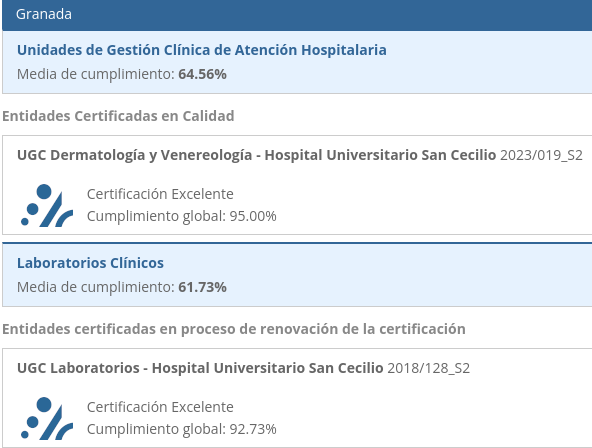
\includegraphics [ width =0.9\textwidth ]{imagenes/Certificado_excelente_hospital_granada.png}
            \caption{Certificación excelente en hospitales de Granada.}
        \end{figure}

        
        
        Por otro lado, si buscamos por ejemplo la unidad que nos interesa para este proyecto, la unidad de neumología, vemos que el hospital Virgen de las Nieves cuenta con un certificado avanzado, además de salir en este artículo de la página mencionada anteriormente, dando alusión a que obtuvo un porcentaje de calidad bastante alto \cite{ElHospit73}:

        \begin{figure}[h]
            \centering
            
\includegraphics [ width =0.7\textwidth ]{imagenes/Certificado_neumologia_hospital.png}
            \caption{Certificación calidad hospital Virgen de las Nieves, neumología.}
        \end{figure}

        \newpage

        \vskip 0.2in
        {\large \textbf{Normativas por las que se rigen las habitaciones de los pacientes.}}
        \vskip 0.2in

        Dentro de las normativas que tiene la ACSA, existe la normativa estándar
        ES 5 08.01\_01 \cite{ACSA_Normativa_habitaciones_hospitales}:

        “Se han definido y se aplican las actuaciones necesarias para
        conocer, registrar y controlar las condiciones de seguridad del
        espacio e instalaciones con los que cuenta la Unidad de Gestión
        Clínica para la realización de su actividad.\cite{ACSA_Normativa_habitaciones_hospitales}”

        Tiene como propósito:

        “Poner en marcha mecanismos para que los responsables de la
        Unidad reciban la información necesaria sobre las condiciones de
        mantenimiento y seguridad de los espacios e instalaciones que dan soporte
        al desarrollo de su actividad, garantizando con el control y seguimiento de
        las posibles incidencias, la seguridad de usuarios y profesionales.\cite{ACSA_Normativa_habitaciones_hospitales}”

    \vskip 0.2in
    {\large \textbf{Cómo son.}}
    \vskip 0.2in
    
    
        Las habitaciones de hospitales principalmente son de dos pacientes, pero puede darse el caso de ser de uno o tres pacientes. Dependiendo del número de pacientes, las medidas varían.\cite{Habitaciones_hospital_medidas}
        
        \begin{itemize}
        	\item Habitaciones individuales(constan de una cama): Las medidas deben de ser sobre unos 10 metros cuadrados (esto varía dependiendo del país, en este caso nos centramos en España, concretamente Andalucía.)\cite{Habitaciones_hospital_medidas}
        	\item Habitaciones dobles(consta de dos camas): Las medidas deben de ser de unos 14 metros cuadrados.\cite{Habitaciones_hospital_medidas}
        	\item Habitaciones triples(constan de 3 camas): Las medidas pueden variar al igual que las anteriores, pero en este caso pueden ser además entre 18 a 20 metros cuadrados.\cite{Habitaciones_hospital_medidas}
        	
         \item Puede darse el caso de que haya habitaciones de cuatro, pero este es el máximo permitido.
         
        \end{itemize} 
        
    \newpage
    \vskip 0.2in
    {\large \textbf{Elementos comunes.}}
    \vskip 0.2in
        Principalmente, nos vamos a centrar en las habitaciones dobles e individuales.
        
        En el caso de las camas, debe de existir una distancia lo suficientemente grande(entre 1 a 1,20 metros) entre las camas y la pared, para poder facilitar la atención al paciente.\cite{Habitaciones_hospital_medidas}
        
        La altura máxima de una habitación es de 2,5 metros.\cite{Habitaciones_hospital_medidas}
        
        Al espacio que hay en la habitación hay que restarle el espacio que ocupan los distintos elementos que hay en esta \cite{Inmobiliario_habitaciones_hospital}:
    
        \begin{itemize}
        	\item Mesillas.\cite{Inmobiliario_habitaciones_hospital_elementos}
        	\item Mesa de cama.\cite{Inmobiliario_habitaciones_hospital_elementos}
        	\item Silla o sillón.\cite{Inmobiliario_habitaciones_hospital_elementos}
        	\item Papeleras.\cite{Inmobiliario_habitaciones_hospital_elementos}
        	\item Sofá de cama para acompañantes.\cite{Inmobiliario_habitaciones_hospital_elementos}
        	\item Tomas de oxígeno y vacío.\cite{Inmobiliario_habitaciones_hospital_elementos}
        	\item Baño.\cite{Inmobiliario_habitaciones_hospital_elementos}
        \end{itemize}

\clearpage

\section{Elementos ambientales en una habitación de hospital.}
\label{sec:elementosAmbientalesHabitacion}
    A continuación se van a mostrar distintos elementos que condicionan el estado de una habitación de hospital.

    \begin{itemize}
    	\item Temperatura.
    		\begin{itemize}
    			\item La temperatura ambiental debe de estar entre unos 20 a 22 grados Celsius, dependiendo de las zonas del hospital varía.\cite{Calidad_Temperatura}
    			\item Se regula por medio de los termostatos que disponen los pacientes.\cite{Calidad_Temperatura}
    			\item Dependiendo del hospital, puede disponer de un sistema de circuito cerrado de ventilación, el cual lleva un sistema que, de manera automática, controla la temperatura.\cite{Calidad_Temperatura}
    		\end{itemize}
    		
    	\item Humedad.
    		\begin{itemize}
    			\item Se considera que está en un umbral adecuado cuando oscila entre el 40 y el 60 por ciento.\cite{Calidad_Humedad}
    			\item En el caso de algunos estados patológicos pulmonares, el grado de humedad relativo bajo oscila entre el 10 y el 20 por ciento, para hacer que el paciente pueda estar en mejores condiciones.\cite{Calidad_Humedad}
    			\item Se controla por medio de higrómetros que se encuentran en las unidades de los pacientes, también hay en pasillos y dependencias especiales.\cite{Calidad_Humedad}
    		\end{itemize}
    	\item Calidad del aire.
    		\begin{itemize}
    			\item La ventilación se realiza abriendo las ventanas y puerta durante breves periodos de tiempo. El tiempo medio es de 10 a 15 minutos.\cite{Calidad_aire}
    			\item La ventilación debe de hacerse de manera que no genere corrientes de aire para que así no sea de manera directa sobre el paciente.\cite{Calidad_aire}
    			\item En los hospitales más modernizados, en caso de tener un circuito cerrado de aire acondicionado, se recomienda evitar abrir las ventanas para ventilar, ya que puede generar descompensaciones en el circuito del aire que está en constante renovación.\cite{Calidad_aire}
    			\item Normalmente, las impurezas que se encuentran en el aire son gases, partículas de polvo y microorganismos.\cite{Calidad_aire}
    		\end{itemize}
            \newpage
    	\item $CO_2$
    		\begin{itemize}
    			\item Los niveles de dióxido de carbono máximos recomendados en interiores debe de estar entre 400 y 800 ppm(partes por millón). \cite{CO2_niveles}
    			\item Para ello es recomendable renovar el aire de las habitaciones, siendo entonces la opción de abrir las ventanas o usando el circuito cerrado de aire en caso de disponer de este.
    		\end{itemize}
    	\item VOC (Volatile Organic Compounds).
    		\begin{itemize}
    			\item Compuestos orgánicos volátiles(COV) que hay en el aire en forma de gas o vapor a temperatura ambiente.\cite{VOC_Niveles}
    			\item Tiene distintas procedencias que pueden generar varios síntomas perjudiciales en los pacientes a través de la respiración y la piel.\cite{VOC_Niveles}
    				\begin{itemize}
    					\item Náuseas.\cite{VOC_Niveles}
    					\item Dolor de cabeza.\cite{VOC_Niveles}
    					\item Mareos.\cite{VOC_Niveles}
    					\item Reacciones alérgicas.\cite{VOC_Niveles}
    				\end{itemize}
    			\item Dependiendo del ppb(partículas por mil millones) puede ser:
    				\begin{itemize}
    					\item De 0 a 200. Muy bueno.\cite{VOC_Niveles}
    					\item De 201 a 600. Bueno.\cite{VOC_Niveles}
    					\item De 601 a 1000. Moderadamente malo.\cite{VOC_Niveles}
    					\item De 1001 a 2000. Muy malo.\cite{VOC_Niveles}
    					\item Más de 2000. Extremadamente perjudicial para la salud.\cite{VOC_Niveles}
    				\end{itemize}
    		\end{itemize}
    	\item $PM2.5.$
    		\begin{itemize}
    			\item Se le denominan a aquellas partículas cuyo diámetro es igual o inferior a 2.5 micras\cite{Definicion_Particulas2.5}. 
    			\item Provienen de fuentes relacionadas con la actividad humana, como emisiones de gases contaminantes de vehículos, industria, agricultura, entre otros. Puede provenir también por gases como $SO_2$, $NO_x$, $NH_3$ y otros compuestos orgánicos volátiles.
    			\item Tienen la particularidad de que son capaces de acceder a los pulmones e incluso alcanzar los alveolos, llevando sustancias perjudiciales a zonas sensibles del aparato respiratorio con riesgo a agravar enfermedades respiratorias.\cite{Calidad_nivel_PM25}
                    \newpage
    			\item Los valores para el $PM2.5$ son:
    			\begin{itemize}
    				\item Bueno: menos de 25 $\mu g/m^3$.\cite{Calidad_nivel_PM25}
    				\item Moderado: Entre 25 y 50 $\mu g/m^3$.\cite{Calidad_nivel_PM25}
    				\item Malo: Entre 50 y 100 $\mu g/m^3$.\cite{Calidad_nivel_PM25}
    				\item Muy malo: Entre 100 y 300 $\mu g/m^3$.\cite{Calidad_nivel_PM25}
    				\item Extremadamente perjudicial: Más de 300 $\mu g/m^3$.\cite{Calidad_nivel_PM25}
    			\end{itemize}
    			\item Por otro lado, los valores legislados por el estándar son:
    			\begin{itemize}
    				\item 25 $\mu g/m^3$ en 24 horas.\cite{Calidad_nivel_PM25}
    				\item 8 $\mu g/m^3$ anuales.\cite{Calidad_nivel_PM25}
    			\end{itemize}
    			\item La manera más adecuada de actuar en estos casos es como en las anteriores, ventilando el espacio del paciente, ya sea mediante el sistema de circuito de ventilación o abriendo las ventanas en caso de no tener el anterior.
    		\end{itemize}
    \end{itemize}
\newpage
\section{Enfermedades pulmonares.}

    En esta sección vamos a estudiar posibles enfermedades que pueden verse afectadas por el mal estado ambiental de la habitación hospitalaria. 
    \\Partiendo de que alguno de los valores que se han mencionado  \hyperref[sec:elementosAmbientalesHabitacion]{en el apartado anterior}.

    \vskip 0.2in
    {\large \textbf{Enfermedad Pulmonar Obstructiva Crónica (EPOC).}}
    \vskip 0.2in
    {\large \textbf{Asma.}}
    \vskip 0.2in
    {\large \textbf{Neumonía.}}
    \vskip 0.2in
    {\large \textbf{Enfermedades cardiovasculares.}}
    \vskip 0.2in
    {\large \textbf{Infecciones nosocomiales.}}
    \vskip 0.2in
    {\large \textbf{Enfermedad de Parkinson.}}
    \vskip 0.2in
    {\large \textbf{Alergias y sensibilidades.}}
    \vskip 0.2in
    {\large \textbf{Enfermedades mentales.}}
    \vskip 0.2in



\section{Medidores.}

    {\large \textbf{Partículas $PM.2.5$}}
    \vskip 0.2in
    {\large \textbf{COV}}
    \vskip 0.2in
    {\large \textbf{Dióxido de nitrógeno.}}
    \vskip 0.2in
    {\large \textbf{Calidad del aire.}}
    \vskip 0.2in
    {\large \textbf{Presión barométrica.}}
    \vskip 0.2in
    {\large \textbf{Ruido.}}
    \vskip 0.2in
%
%\input{capitulos/02_EspecificacionRequisitos}
%
%\input{capitulos/03_Planificacion}
%
%\input{capitulos/04_Analisis}
%
%\input{capitulos/05_Diseno}
%
%\input{capitulos/06_Implementacion}
%
%\input{capitulos/07_Pruebas}
%
%\input{capitulos/08_Conclusiones}
%
%%\chapter{Conclusiones y Trabajos Futuros}
%
%
%%\nocite{*}
%\bibliography{bibliografia/bibliografia}\addcontentsline{toc}{chapter}{Bibliografía}
%\bibliographystyle{miunsrturl}

\bibliography{bibliografia/bibliografia}
\addcontentsline{toc}{chapter}{Bibliografía}
\bibliographystyle{unsrt}

%
%\appendix
%\input{apendices/manual_usuario/manual_usuario}
%%\input{apendices/paper/paper}
%\input{glosario/entradas_glosario}
% \addcontentsline{toc}{chapter}{Glosario}
% \printglossary
\chapter*{}
\thispagestyle{empty}

\end{document}
